\documentclass[12pt]{article}
\usepackage[margin=0.75in]{geometry}
\geometry{a4paper}
\usepackage[T1]{fontenc} % Support Icelandic Characters
\usepackage[utf8]{inputenc} % Support Icelandic Characters
\usepackage{graphicx} % Support for including images
\usepackage{hyperref} % Support for hyperlinks
\usepackage{wrapfig}

\usepackage{algorithm}
\usepackage{algorithmicx}
\usepackage{listings}
\usepackage{color}
\usepackage{siunitx}

\usepackage[svgnames]{xcolor}

\usepackage{amsmath}
\usepackage{tikz}
\usetikzlibrary{arrows,automata}

\usepackage{tikz}
\usepackage{tikz-dependency}
\usepackage[spanish,es-noshorthands]{babel}

\usepackage[spanish]{babel}
\usepackage[latin1]{inputenc}
\usepackage[usenames]{color}

\definecolor{mGreen}{rgb}{0,0.6,0}
\definecolor{mGray}{rgb}{0.5,0.5,0.5}
\definecolor{mPurple}{rgb}{0.58,0,0.82}
\definecolor{backgroundColour}{rgb}{0.95,0.95,0.92}

\usepackage{xcolor}

\usepackage{listings}             % Include the listings-package
\lstdefinestyle{CStyle}{
    backgroundcolor=\color{backgroundColour},   
    commentstyle=\color{mGreen},
    keywordstyle=\color{blue},
    numberstyle=\tiny\color{mGray},
    stringstyle=\color{red},
    basicstyle=\footnotesize,
    breakatwhitespace=false,         
    breaklines=true,                 
    captionpos=b,                    
    keepspaces=true,                 
    numbers=left,                    
    numbersep=5pt,                  
    showspaces=false,                
    showstringspaces=false,
    showtabs=false,                  
    tabsize=2,
    language=C
}



%------------------------------------------------------------------
% TITLE
%------------------------------------------------------------------

\title{
\centerline{
    
\includegraphics[width=75mm]{unsa.png}}
    \vspace{0.5 cm}
        Teoría de la Computación - Laboratorio A
        \\
        \\
        \\
        \textbf{Práctica de Laboratorio #6} 
        \large  
        \\
        %SC-T-718-ATSR,Automatic Speech Recognition, 2019-1 
        %\\ 
        \small Universidad Nacional de San Agustín - Escuela Profesional de Ingeniería de Sistemas, Arequipa, Perú 
  }

\author{
    Carlos Alberto Mestas Escarcena
    \\
    \texttt{cmestas@unsa.edu.pe}
}

\date{23 de Junio del 2020}

\begin{document}

\maketitle

\section{Describir que pasa si no se considera el carácter “.” en el analizador léxico}

Analiza lo que ingresemos, porque el caracter “.” sirve para reconocer el resto de símbolos que no formen parte del analizador léxico, por ejemplo si en nuestro analizador léxico programamos para que reconozca solo “abc”, al momento de nosotros ejecutar el programa si nosotros ingresamos abc, no habría ningún problema, pero en caso de que por ejemplo ingresemos “abcd” el programa nos diría que se reconoció abc, pero en la impresión también aparecería el caracter “d”. 

\section{¿Cual es el mejor lugar para definir la función main, en el lexer o en el parser? ¿Porque?}

En el parser, porque el lexer realiza un parsing a bajo nivel convirtiendo caracteres o secuencias de caracteres en tokens, el parser es responsable de agrupar los tokens en agrupaciones de acuerdo con reglas gramaticales, por ejemplo, construir identificadores y operadores en expresiones.

\section{Crear un programa que solo reconozca “bb”}

\begin{lstlisting}[language=bash,frame=single,style=CStyle,caption={lexicoExercise3.l}]
%{
    #include "sintacticoExercise3.tab.h"
%}

%%
bb         {return (bb);}
\n         {return (EOL);}
.          {return yytext[0];}
%%

int yywrap(){
    return 0;
}
\end{lstlisting}

\begin{lstlisting}[language=bash,frame=single,style=CStyle,caption={sintacticoExercise3.y}]
%{
    #include <stdio.h>
    #include <stdlib.h>
    int yylex();
    int yyerror(char* s);
%}
%token bb
%token EOL
%%

c: bb EOL        {printf("Se reconocio la cadena bb\n");
                    exit(0); }
;

%%

int yyerror(char* s){
    printf(" Error sintactico: %s \n",s);
    exit(0);
}

void main(){
    printf("Ingrese una cadena: \n");
    yyparse();
    yylex();
}
\end{lstlisting}

\clearpage
\newpage

\begin{figure}[h]
    \centering
    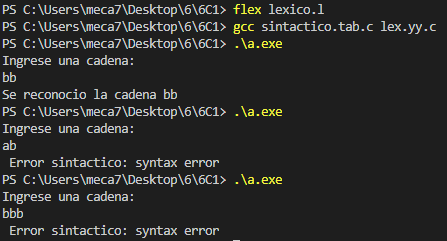
\includegraphics[width=0.62\textwidth]{images/Capture003A.PNG}
    \caption{Ejemplo ejecuciones}
\end{figure}

\section{Crear un programa que haga la operación asignación de valor a una variable}

Para el desarrollo de este ejercicio, podemos ver distintas formas de como asignar valor a una variable en C:

\begin{figure}[h]
    \centering
    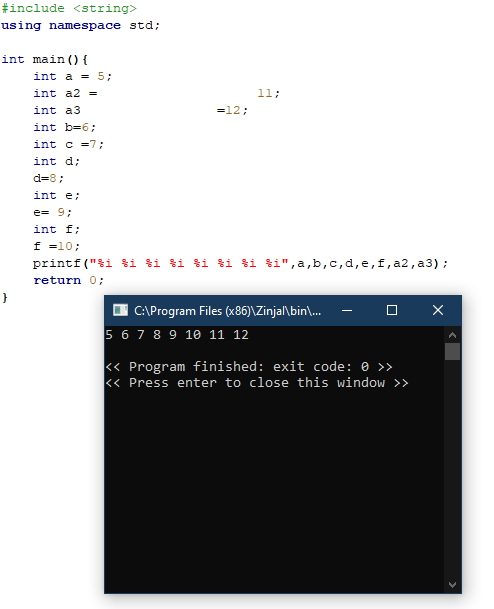
\includegraphics[width=0.5\textwidth]{images/CaptureZinjai.PNG}
    \caption{Ejemplo asignación de variables int}
\end{figure}


\clearpage
\newpage

\begin{lstlisting}[language=bash,frame=single,style=CStyle,caption={lexico.l}
%{
    #include "sintactico.tab.h"
%}
number [0-9]+
word [a-zA-Z]+
space [ \t]
%%
int              {return (INT);}
{word}           {return (WORD);}
-?{number}       {return (NUMBER);}
;                {return (SYMBOL1);}
=                {return (SYMBOL2);}
{space}+         {return (SPACE);}  
\n               {return (EOL);}
.                {return yytext[0];}
%%

int yywrap(){
    return 0;
}
\end{lstlisting}

\begin{lstlisting}[language=bash,frame=single,style=CStyle,caption={sintactico.y}]
%{
    #include <stdio.h>
    #include <stdlib.h>
    int yylex();
    int yyerror(char* s);
%}
%token INT 
%token WORD
%token NUMBER
%token SYMBOL1
%token SYMBOL2
%token SPACE
%token EOL
%%

s:  INT SPACE WORD d EOL        {printf("Se reconocio el ingreso de variable entera\n");
                                    exit(0); }
;
d:  e | f 
;
e:  SYMBOL1 EOL WORD SPACE SYMBOL2 SPACE NUMBER SYMBOL1 | SYMBOL1 EOL WORD SYMBOL2 NUMBER SYMBOL1 | SYMBOL1 EOL WORD SYMBOL2 SPACE NUMBER SYMBOL1 | SYMBOL1 EOL WORD SPACE SYMBOL2 NUMBER SYMBOL1  
;
f:  SPACE SYMBOL2 SPACE NUMBER SYMBOL1 | SYMBOL2 SPACE NUMBER SYMBOL1 | SPACE SYMBOL2 NUMBER SYMBOL1 | SYMBOL2 NUMBER SYMBOL1
;
%%

int yyerror(char* s){
    printf(" Error sintactico: %s \n",s);
    exit(0);
}

void main(){
    printf("Ingrese una asignacion de variable para el lenguaje C: \n");
    yyparse();
    yylex();
}
\end{lstlisting}

\clearpage
\newpage

\begin{figure}[h]
    \centering
    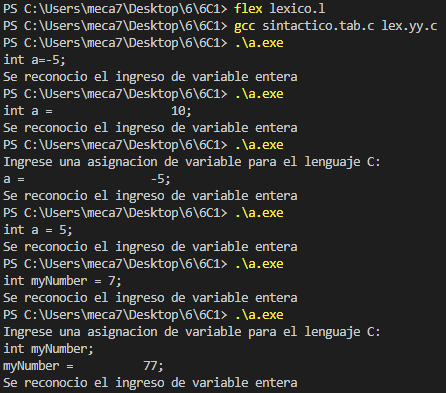
\includegraphics[width=0.62\textwidth]{images/Capture004A.PNG}
    \caption{Ejemplo ejecución - Ejercicio 4 - Parte 1}
\end{figure}

\begin{figure}[h]
    \centering
    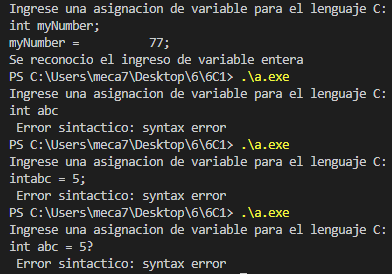
\includegraphics[width=0.62\textwidth]{images/Capture004B.PNG}
    \caption{Ejemplo ejecución - Ejercicio 4 - Parte 2}
\end{figure}
    
\end{document}